\documentclass[12pt]{article}

% URLs and hyperlinks ---------------------------------------
\usepackage{hyperref}
\hypersetup{
colorlinks=true,
linkcolor=blue,
filecolor=magenta,      
urlcolor=blue,
}
\usepackage{xurl}
%---------------------------------------------------

\usepackage{float}
\usepackage{adjustbox}
\usepackage{graphicx}
\usepackage{rotating}
\usepackage{mathtools}
\usepackage{enumitem}
\usepackage{gensymb}

\usepackage{xepersian}
\settextfont{Yas}
\setdigitfont{Yas}

\title{	گزارش کار آزمایش ششم \\ مدار‌های \lr{RLC}
}
\author{	گروه: \\	اریسا احسانی \\	سید حسین حسینی \\	مهدی حق‌وردی \\ \\	شعبه شش
}
\date{}
\renewcommand{\arraystretch}{1.4}

\begin{document}
\maketitle
\tableofcontents
\clearpage

\section{آزمایش}

\subsection{}
مداری مطابق شکل مقابل ببندید و با فرکانس ۱ کیلوهرتز محاسبات را آغاز کنید.

\begin{figure}[H]
\begin{center}
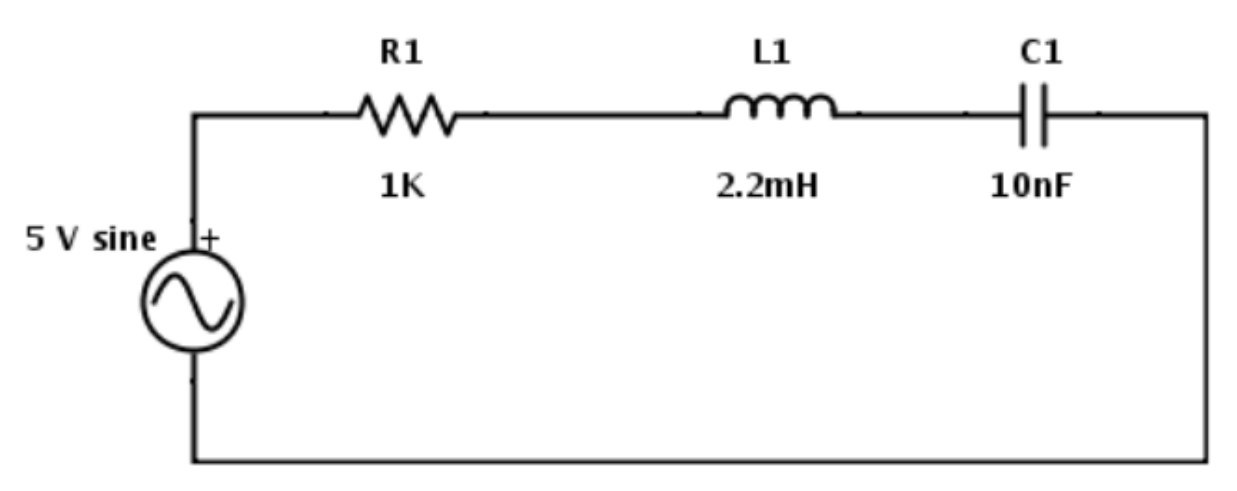
\includegraphics[width=0.9\textwidth, height=5cm]{./images/6.1}
\end{center}
\end{figure}

\begin{figure}[H]
\begin{center}
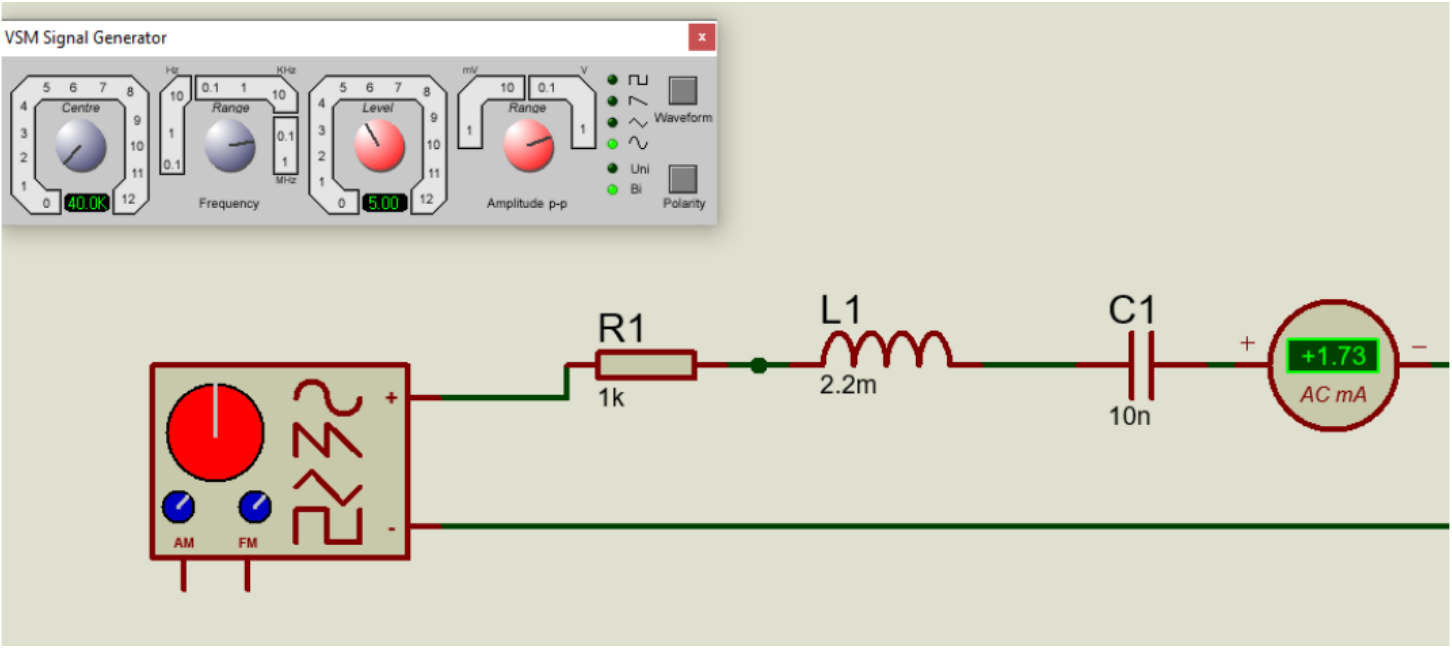
\includegraphics[width=0.9\textwidth, height=5cm]{./images/6.1.a}
\end{center}
\end{figure}

\begin{figure}[H]
\begin{center}
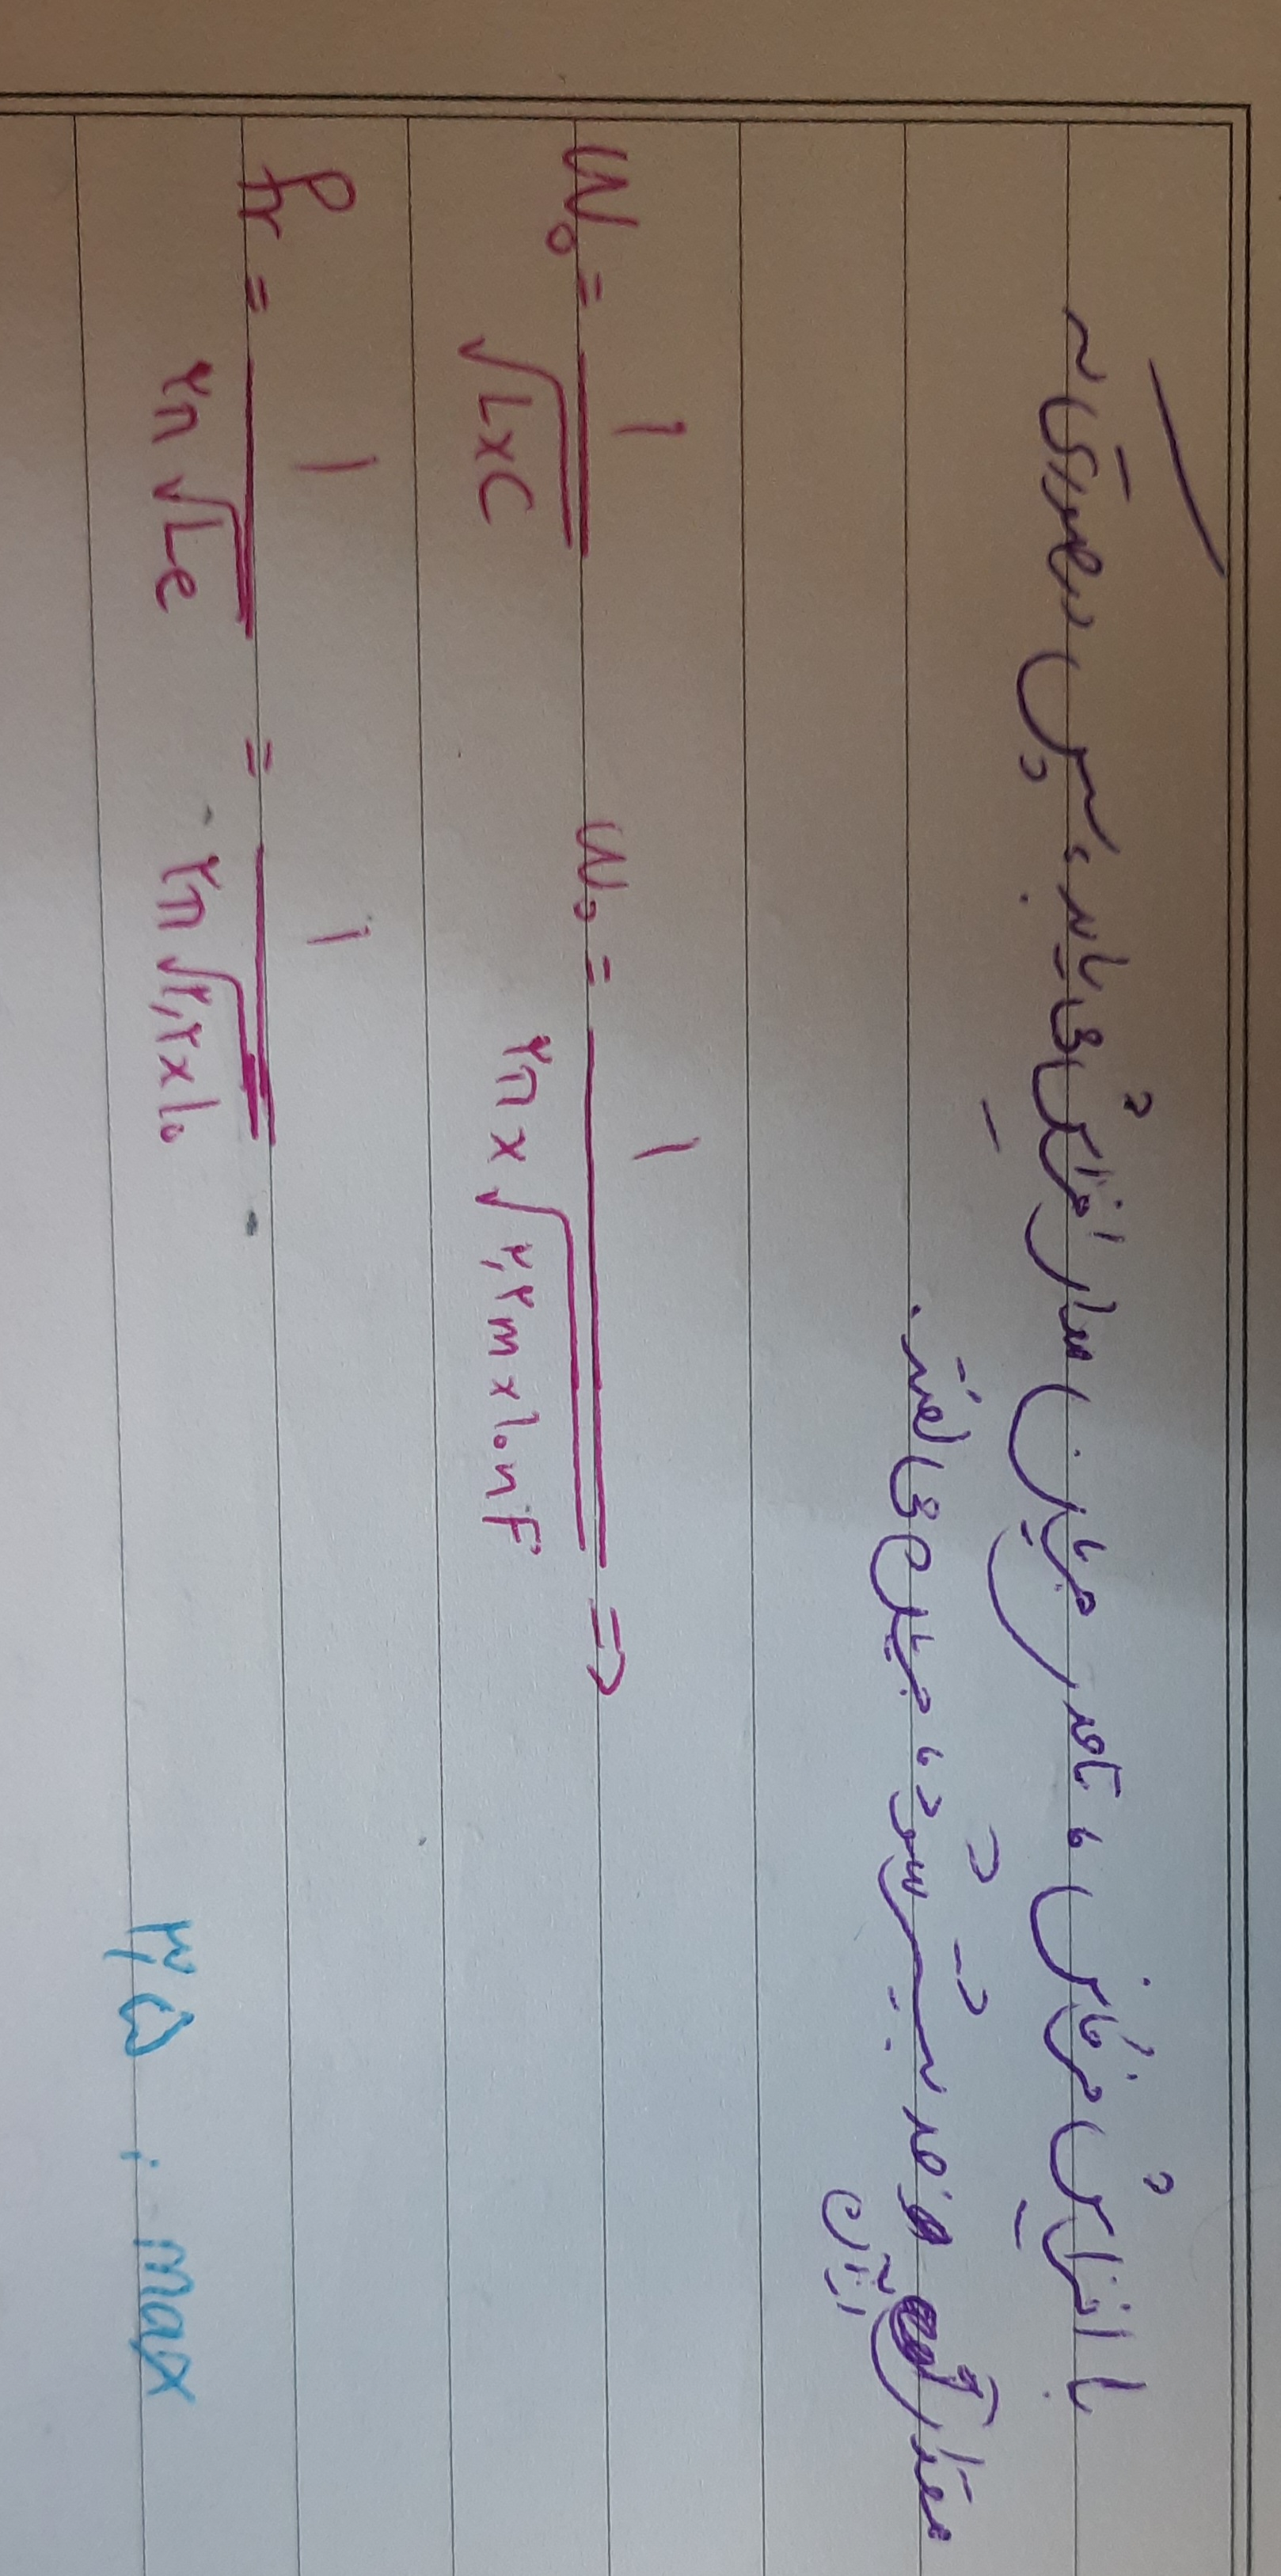
\includegraphics[width=5cm, height=0.9\textwidth, angle=90]{./images/6.1.aa}
\end{center}
\end{figure}

\clearpage
\subsection{}
یک آمپرمتر به صورت سری با مدار قرار دهید و در هنگامی که حداکثر دامنه را داریم مقدار جریان را بدست آروید. آیا اعداد بدست آمده با مباحث نظریه مطرح شده هماهنگی دارند؟ توضیخ مختصری در گزارش کار خود در این رابطه قرار دهید.

\begin{figure}[H]
\begin{center}
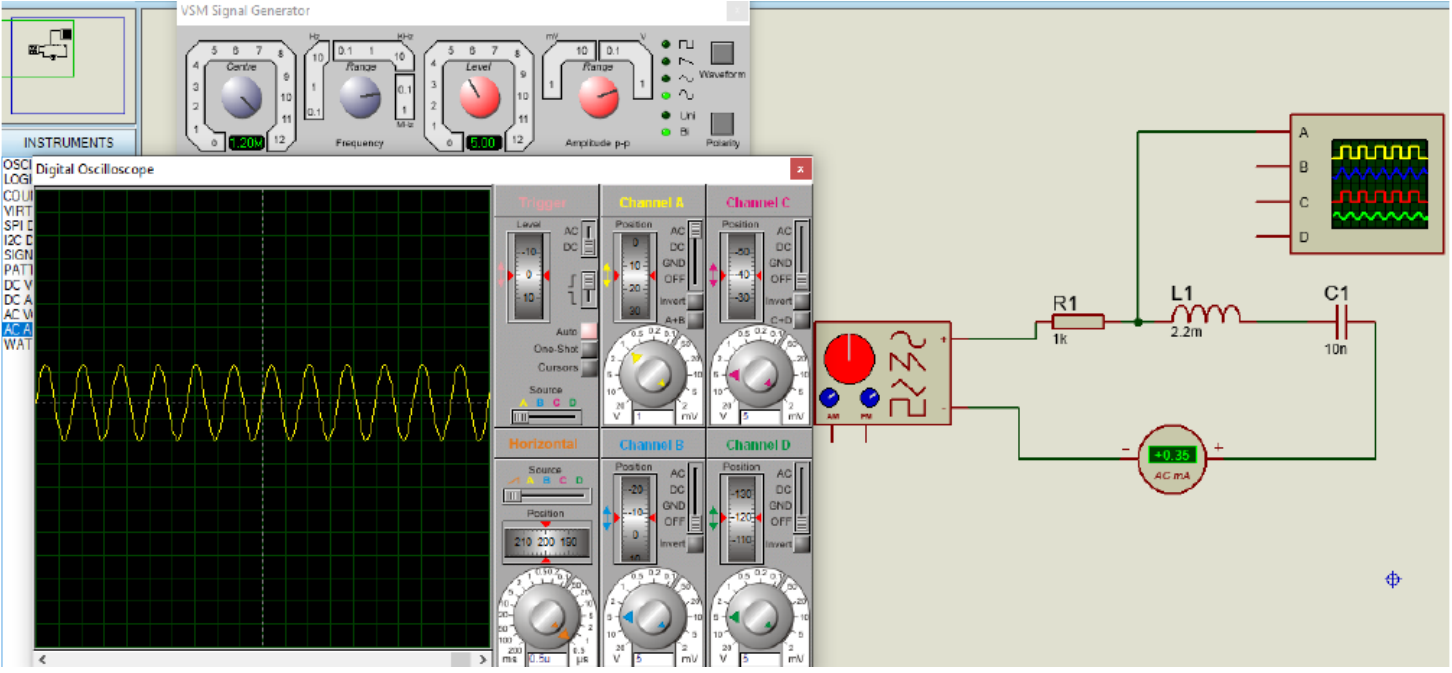
\includegraphics[width=0.9\textwidth, height=5cm]{./images/6.2.a}
\end{center}
\end{figure}

حداکثر دامنه تقریبا برابر با $3.5$ بلوک است.

حداکثر جریان $0.14$ میلی آمپر است.

جریان بدست آمده با مقدار نظری حدودا برابر است. 

\clearpage
\subsection{}
یک مدار \lr{RLC} با مقدار سلف ۱۸ میلی هانری و خازن $3.3$ نانو فاراد و پتانسیومتر ۱۰ کیلو اهم بسازید و ولتاژ پیک تا پیک ۴ ولت به صورت مربعی به مدار بدهید و خروجی را از خازن مشاهده کنید (فرکانس را ۱ کیلوهرتز در نظر بگیرید.)						مقاومت را تغییر دهید، سه حالت پاسخ گذرای مدار را بررسی کیند و اشکال آن را روی اسیلوسکوپ مشاهده کنید و مقدار مقاومت بحرانی را بیابید؛ همچنین ثابت زمانی و ضریب میرایی مدار را در حالت میرایی بحرانی را اندازه بگیرید.


\begin{figure}[H]
\begin{center}
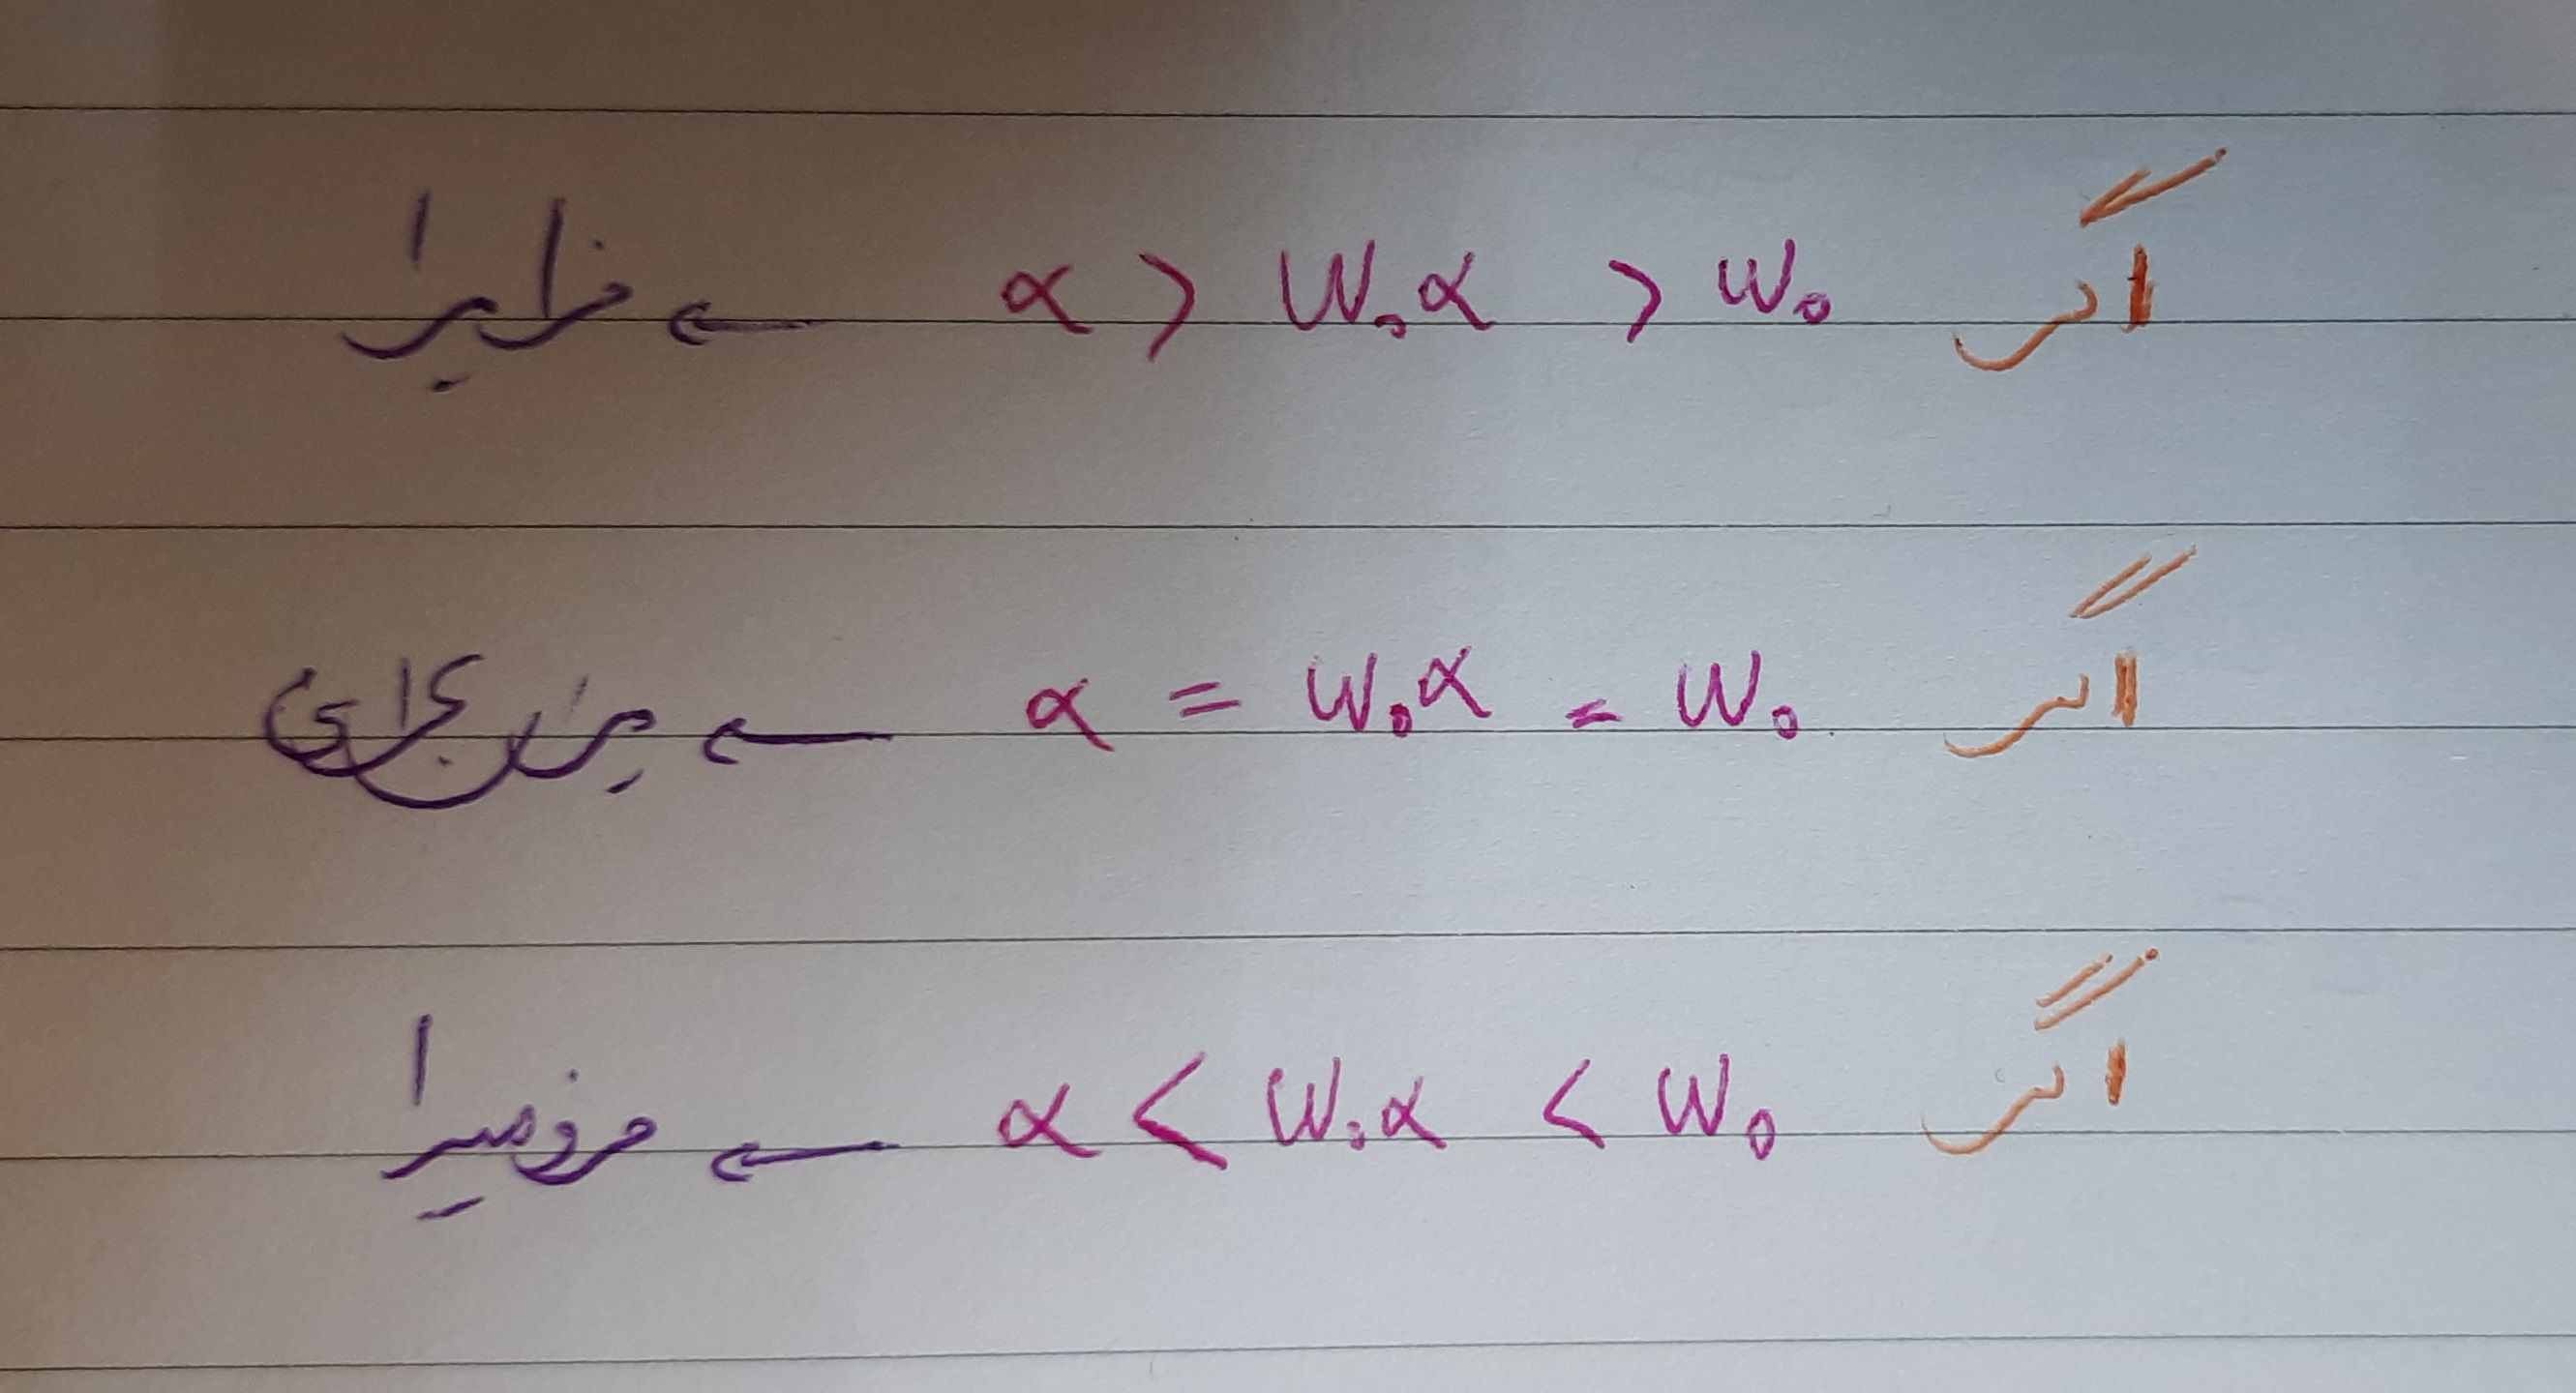
\includegraphics[width=0.9\textwidth, height=6cm]{./images/6.4.a}
\end{center}
\end{figure}

\begin{figure}[H]
\begin{center}
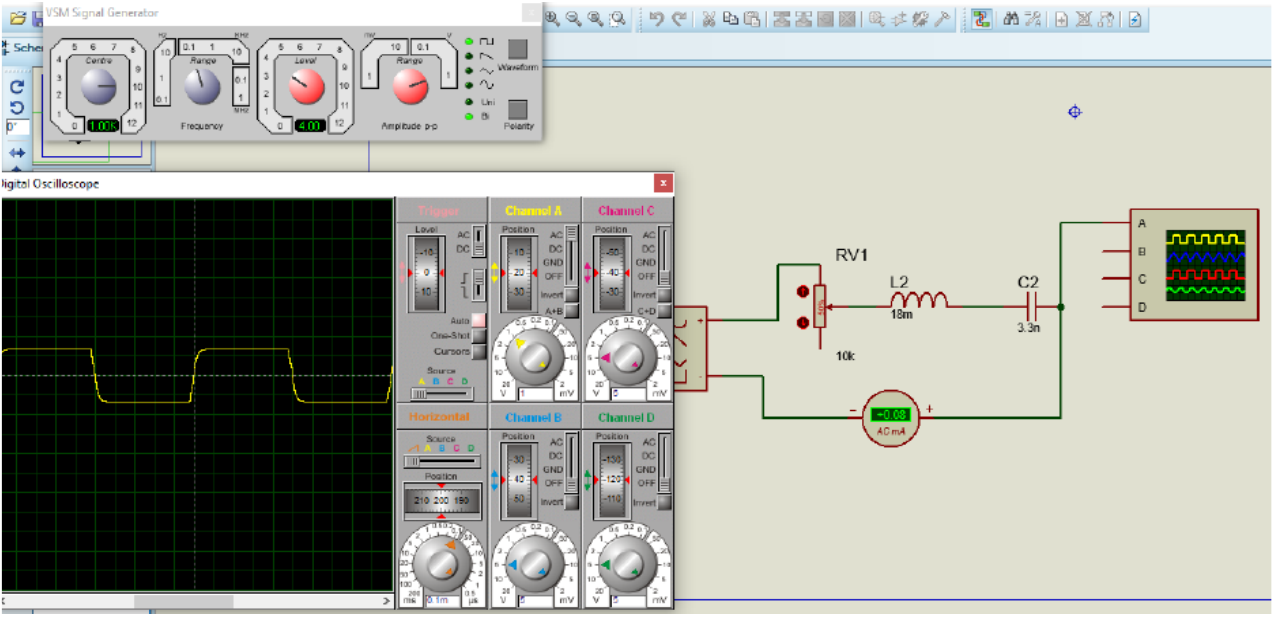
\includegraphics[width=0.9\textwidth, height=6cm]{./images/6.3.a.1}
\end{center}
\end{figure}
\begin{figure}[H]
\begin{center}
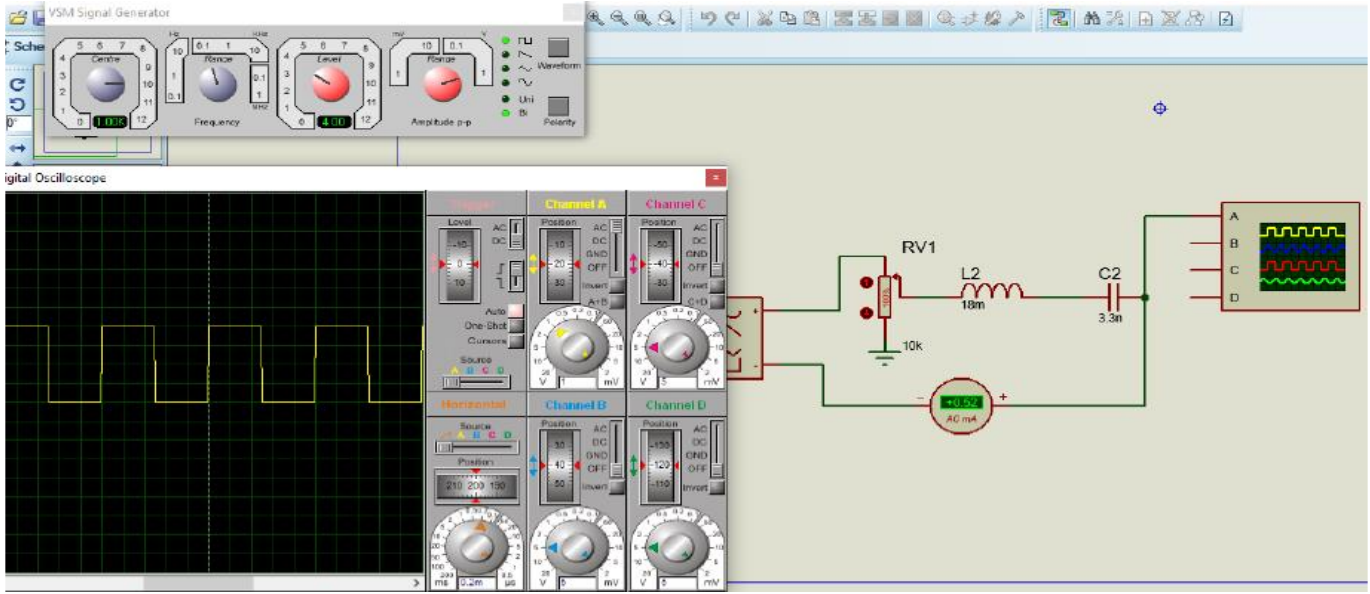
\includegraphics[width=0.9\textwidth, height=6cm]{./images/6.3.a.2}
\end{center}
\end{figure}
\begin{figure}[H]
\begin{center}
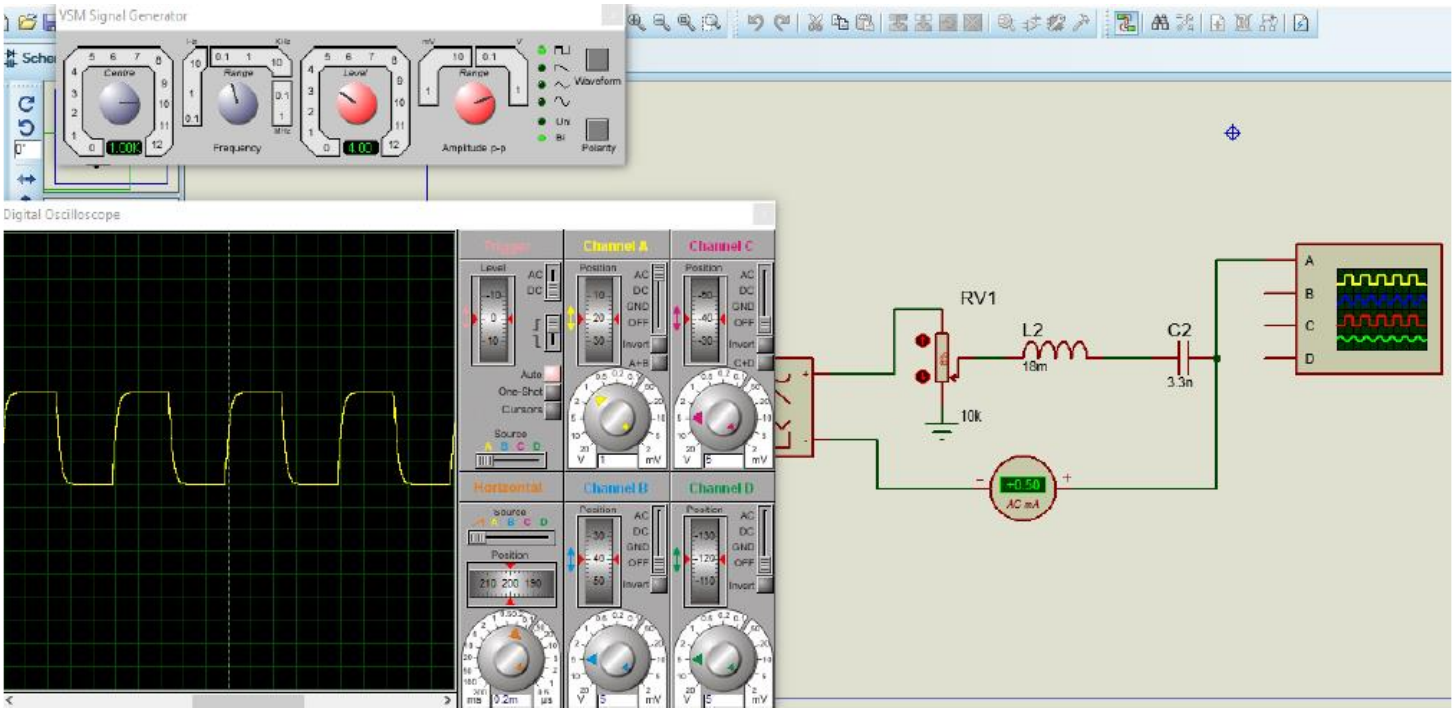
\includegraphics[width=0.9\textwidth, height=6cm]{./images/6.3.a.3}
\end{center}
\end{figure}

\clearpage
\subsection{}
مداری مطابق شکل زیر را ببندید. از اعداد قسمت ۳ استفاده کنید. از پتانسیومتر ۱۰ کیلو استفاده کنید.						جدول را تکمیل کنید

\begin{figure}[H]
	\begin{center}
		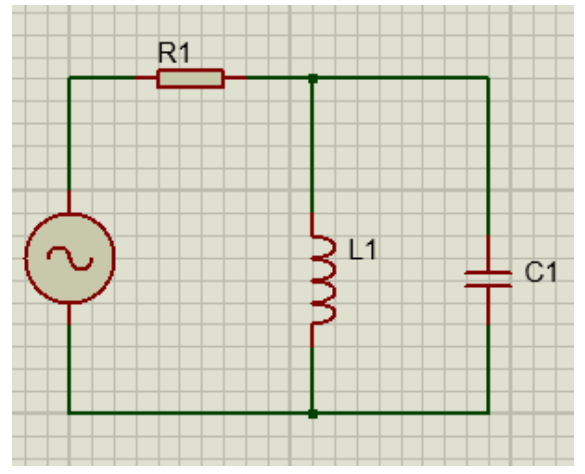
\includegraphics[width=0.9\textwidth, height=7cm]{./images/6.4}
	\end{center}
\end{figure}

\begin{figure}[H]
\begin{center}
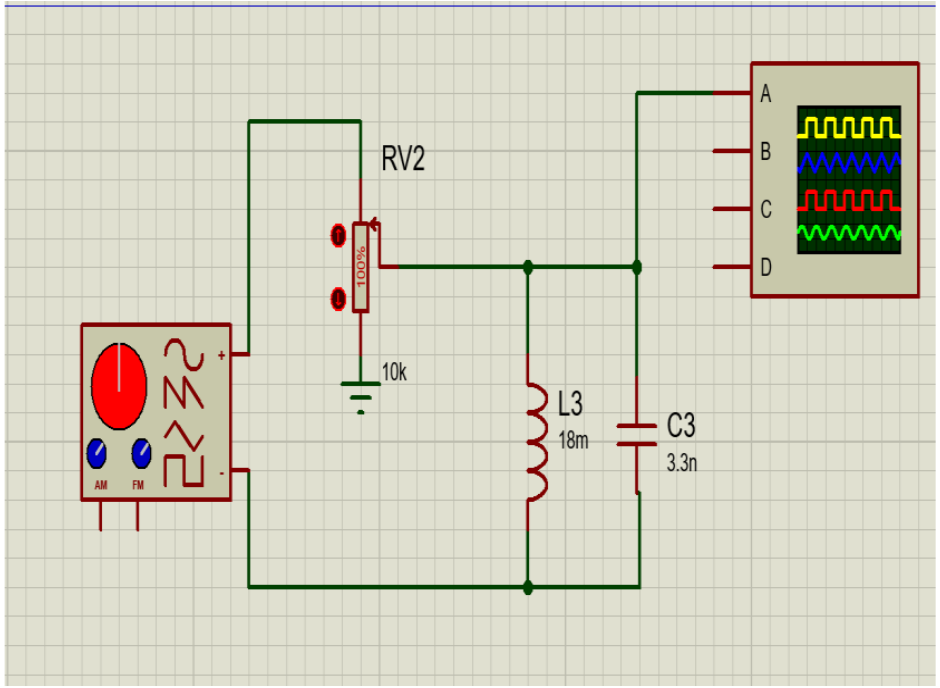
\includegraphics[width=0.9\textwidth, height=7cm]{./images/6.4.a.1}
\end{center}
\end{figure}

\begin{figure}[H]
\begin{center}
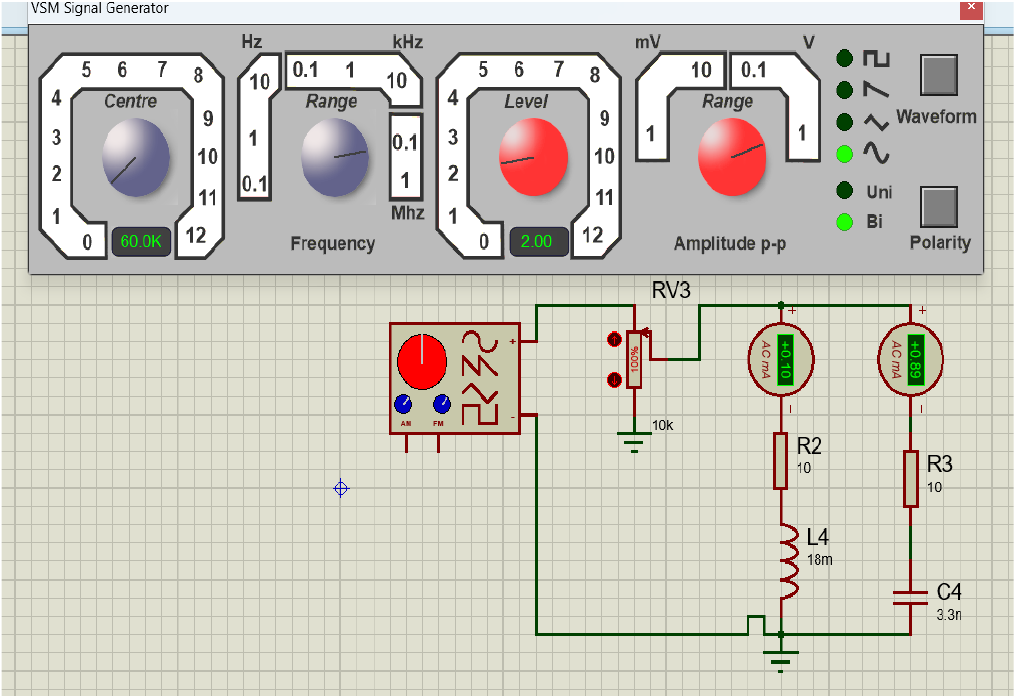
\includegraphics[width=0.9\textwidth, height=7cm]{./images/6.4.a.2}
\end{center}
\end{figure}

در شکل بالا بیشترین دامنه برابر ۲ ولت است و همچنین فیلتر میانگذر است.

\clearpage
\subsection{}
مدار مرتبه دوم سری با خازن $0.1$ میکرو فاراد و سلف ۲۵ میلی هانری و مقاومت ۲۲۰ اهم ببندید. فرکانس تشدید را پیش‌بینی کنید.



\begin{figure}[H]
\begin{center}
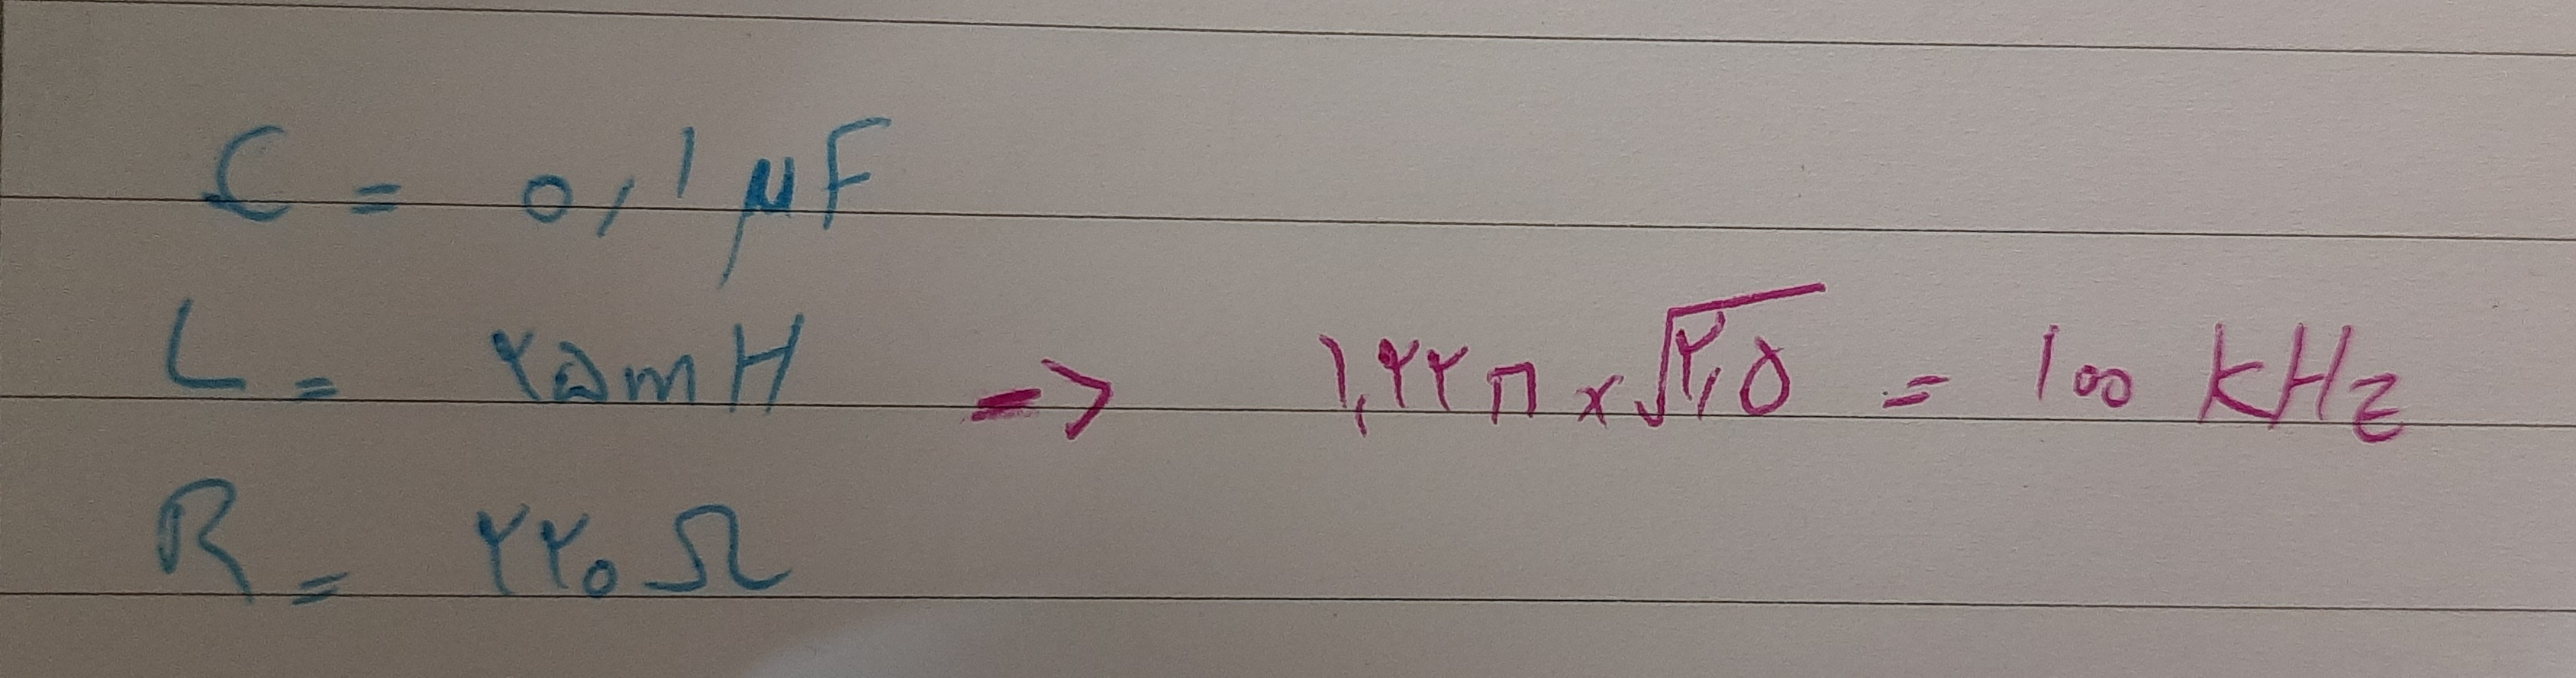
\includegraphics[width=\textwidth, height=5cm]{./images/6.5.a}
\end{center}
\end{figure}

\begin{latin}
\begin{table}[H]
\begin{adjustbox}{width=\textwidth}
\begin{tabular}{|c|c|c|c|c|c|}
\hline
Frequency (HZ) & 
$V_L(p - p)$ & 
$V_c(p - p)$ & 
$V_R(p - p)$ & 
$l_{p - p} = \frac{V_R(p - p)}{R}$ & 
$Z_r = \frac{V_{p - p}}{l_{p - p}}$ \\
\hline
\hline
500 & 0.1 & 3 & 0.05 & 11 & 88 \\
\hline
1000 & 0.5 & 3.2 & 0.5 & 110 & 880 \\
\hline
1500 & 1 & 4 & 1.1 & 242 & 1936 \\
\hline
2000 & 2.9 & 6 & 2.2 & 484 & 3872 \\
\hline
2500 & 5 & 9 & 4.9 & 1078 & 8624 \\
\hline
3000 & 8.5 & 11 & 8.5 & 1870 & 14960 \\
\hline
3500 & 9 & 10 & 9.5 & 2090 & 16720 \\
\hline
4000 & 7.5 & 8 & 7.2 & 1584 & 12672 \\
\hline
4500 & 6.8 & 6.4 & 6.5 & 1430 & 11440 \\
\hline
5000 & 5 & 5.4 & 5.8 & 1276 & 10208 \\
\hline
5500 & 5.3 & 5 & 5 & 1100 & 8800 \\
\hline
\end{tabular}
\end{adjustbox}
\end{table}
\end{latin}

\clearpage
\subsection{}
مداری مطابق شکل زیر ببندید و سپس جدول را کامل کنید

\begin{figure}[H]
\begin{center}
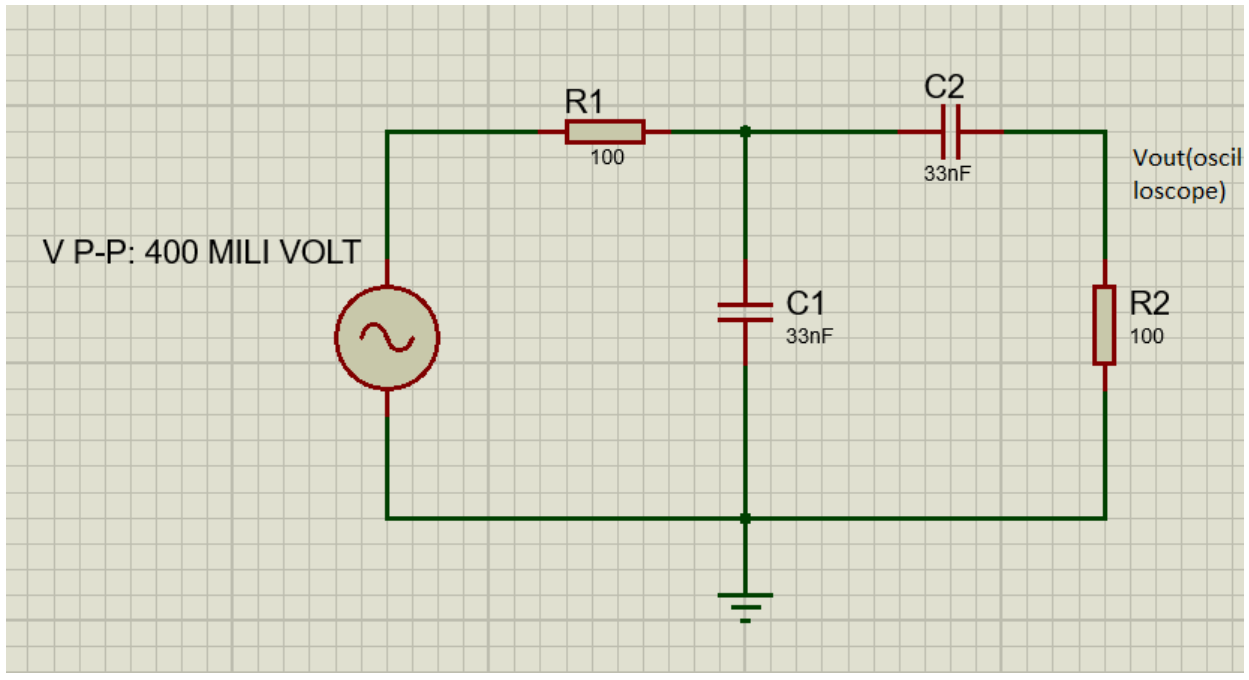
\includegraphics[width=\textwidth, height=6cm]{./images/6.6}
\end{center}
\end{figure}

\begin{figure}[H]
\begin{center}
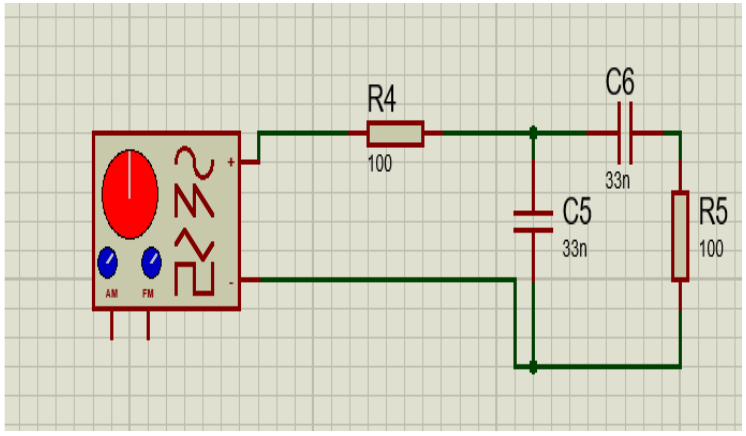
\includegraphics[width=\textwidth, height=6cm]{./images/6.6.a}
\end{center}
\end{figure}

\begin{latin}
\begin{table}[H]
\begin{adjustbox}{width=\textwidth}
\begin{tabular}{|c|c|c|c|c|c|c|c|c|c|c|c|c|c|c|c|}
\hline
F (HZ) & 
100 & 
200 & 
300 & 
500 & 
1K & 
2K & 
5K & 
10K & 
20K & 
50K & 
100K & 
150K & 
200K & 
250K & 
300K \\
\hline
\hline
$V_0$ & 0 mV & 2.5 mV & 3 mV &  5 mV & 10 mV & 20 mV & 
40 mV & 70 mV & 
100 mV & 100 mV & 90 mV & 
70 mV & 60 mV & 50 mV & 40 mV \\
\hline
\end{tabular}
\end{adjustbox}
\end{table}
\end{latin}

\clearpage
\subsection{}
مداری مطابق شکل زیر ببندید و سپس جدول را کامل کنید.

\begin{figure}[H]
\begin{center}
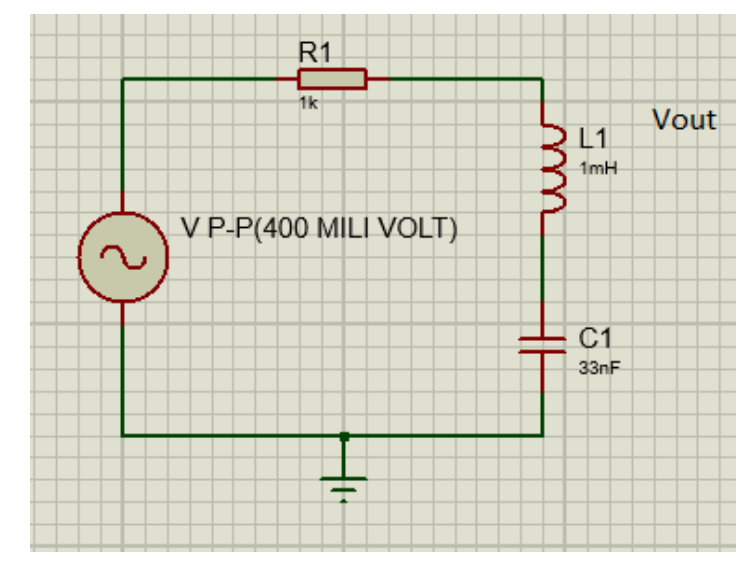
\includegraphics[width=7cm, height=5cm]{./images/6.7}
\end{center}
\end{figure}

\begin{figure}[H]
\begin{center}
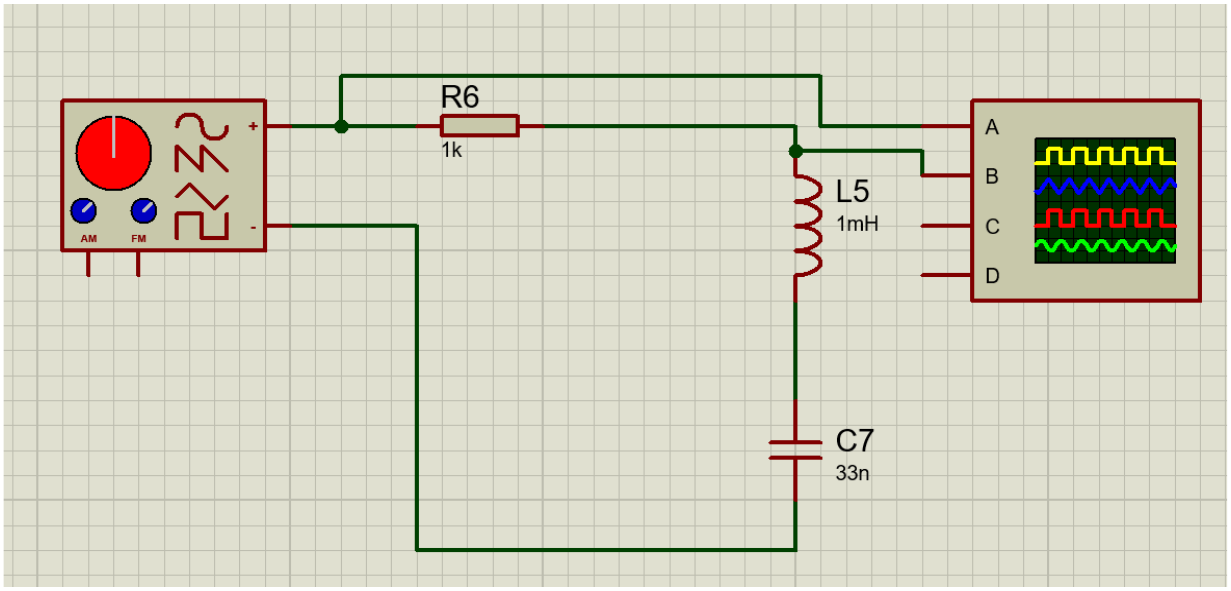
\includegraphics[width=7cm, height=5cm]{./images/6.7.a}
\end{center}
\end{figure}

\begin{latin}
\begin{table}[H]
\begin{adjustbox}{width=\textwidth}
\begin{tabular}{|c|c|c|c|c|c|c|c|c|c|c|c|c|c|c|c|}
\hline
F (HZ) & 
100 & 
200 & 
300 & 
500 & 
1K & 
2K & 
5K & 
10K & 
20K & 
50K & 
100K & 
150K & 
200K & 
250K & 
300K \\
\hline
\hline
$V_0$ & 400 mV & 400 mV & 400 mV & 400 mV & 400 mV & 350 mV & 
260 mV & 150 mV & 40 mV & 100 mV & 200 mV & 
300 mV & 350 mV & 400 mV & 400 mV \\
\hline
\end{tabular}
\end{adjustbox}
\end{table}
\end{latin}
\end{document}